\documentclass[book,with-crop]{laspex}

\newcommand{\spextitel}{Echnaton}
\newcommand{\ellertitel}{Känd från Tebe}
\newcommand{\korttitel}{Ech.}

\newcommand{\am}{\replik{Amenhotep}}
\newcommand{\nef}{\replik{Nefertite}}
\newcommand{\tut}{\replik{Tutanchamon}}
\newcommand{\cha}{\replik{Chabba}}
\newcommand{\anc}{\replik{Anchesenpaaton}}
\newcommand{\pt}{\replik{Prästen}}
\newcommand{\pa}{\replik{Prästinnan}}

\usepackage{blindtext} % Just for test

\begin{document}

\iffalse
\begin{onepage}
Denna sida borde ligga först!
\end{onepage}
\thispagestyle{plain}
\clearpage
\fi

\akt{I Faraos audienssal}

\musikbox{Stämningssättande dans}{Dansare \& kamel}{Ur Aladdin}{Menken}{En beskrivning som vanligtvis inte används i bokformatet. Det syns inte ens i boken!}{Eller en undertitel}

\scenanvisning{Amenhoteps tron står mitt på bakre delen av scenen. Templet har inget tak och morgonsolen skiner in mellan pelarkolonnerna.}

\scen{Slaven blir omkullvält}

\scenanvisning{Tutanchamon springer över scenen och välter omkull tjänaren Chabba som kommer förbi med Faraos frukost. Denne tappar då saker, bland annat ett par ägg.}

\scen{Drömmar om silvertejp, drömmar om guldåldrar}



\scenanvisning{Anchesenpaaton och Nefertite kommer in.}

\nef      \hur{Trött, som i Emil} Tutanchamon, förgrömmade unge!

\anc    Mamma, att min bror skulle bli kung e\dots
        \hur{Konstpaus för att hitta diplomatiskt uttryck}
        \dots svårtänkbart -- men vi är ju i alla fall förlovade.

\nef      \hur{Sarkastiskt} Nåja, det finns ju de som är än mer obegåvade.

\scenanvisning{De tittar på slaven, som famlar på golvet efter frukosten.}

\forts  En drottning som jag ska vara god mot sina slavar\dots
        Jag kan inte alltid vara filantrop.

\anc    Han får skylla sig själv som snavar
        -- han borde ha läst sitt horoskop.

\nef      Du må vara astrologikursens största stjärna
        men jag tror att prästerna börjar vända upp och ner på din hjärna.

\anc    Nu känner jag negativa energier strömma\dots
        Du behöver zonkristallakupunktur!

\scenanvisning{Anchesenpaaton gör ett försök att hela Nefertite, men Nefertite är inte intresserad.}

\nef    Anchesenpaaton, sluta drömma!
        Du borde ägna dig åt att optimera vår infrastruktur;
        \hur{Blir exalterad, glömmer Anchesenpaaton}
        vägnät, broar, eller en handelsflotta\dots{}

\anc    Nej mamma, teknik är bara för nördar!

\nef      \dots{} eller dämma upp Nilen för att ge oss bättre skördar!

\anc    Det är så tråkigt att räkna och måtta.

\musikbox{Pseudovetenskap och ingenjörskonst}{Anchesenpaaton \& Nefertite}{Pappa jag vill ha en italienare ur Stinsen brinner}{Galenskaparen Eriksson}{}

\begin{onepage}
\label{pseudoI}%
\sanglada{%
\rubrik{Pseudovetenskap och ingenjörskonst}
\begin{sangtext}
\sangare{Nef}%
    Lyssna och lyd, din attityd
	är inte sober.
	Prästen med fru lurar dig ju,
	de är teknofober.
	Astrologi, telepati
	är för de veka.
	Var lite sund, skaffa en grund,
	lär dig meka!\radskip

\sangare{Anc}%
    Jag vill bli befriad från materien,
	sväva bland andar och själar.
	Jag vill bli befriad och jag ber igen.
	Släpp tekniksamhällets trälar!
	Jag vill bli befriad från materien,
	uppleva drömfantasier!
	Jag vill bli befriad och jag ser, min vän.
	grå är alla teorier!\radskip
	
	Åh, du gamla dumma moder,
	skippa logiska metoder!
	Dina gudar gråter floder.
	Lösgör ditt roder!\radskip
	
\sangare{Nef}%
    Du har lärt dig fel och om det sker igen,
	får du läsa extra under ferien!\radskip
	
\sangare{Anc}%
    Jag vill bli befriad från materien!\radskip
	
\hfill\emph{Text: Tore K}
\end{sangtext}
\begin{sangtextsingel}
\emph{Pappa jag vill ha en italienare}\hfill\textsc{Musik: Galenskaparna, Arr: Karin S-A}
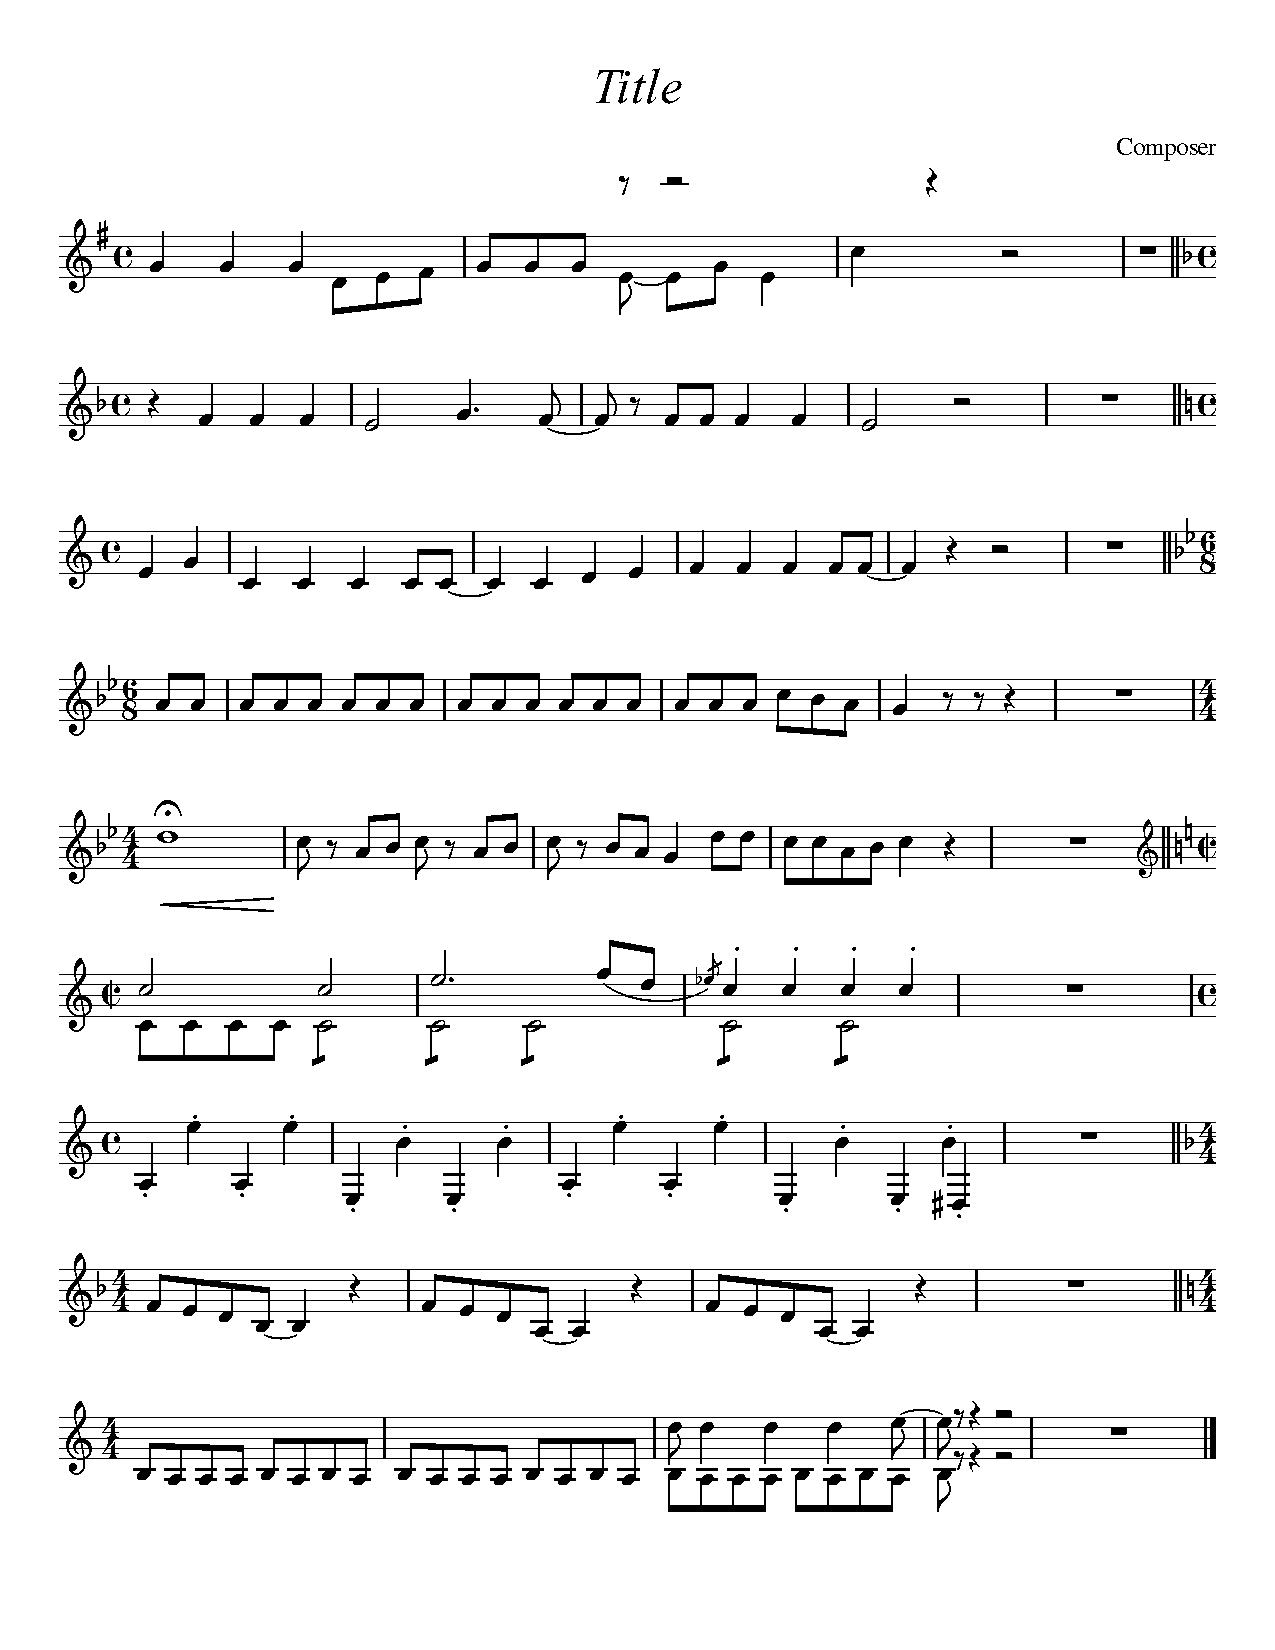
\includegraphics[height=1.60cm, clip,%
trim=1.05cm 22.5cm 5.9cm 3.5cm]{songs/noter_ovr1.pdf}
\end{sangtextsingel}}
\end{onepage}

%\musik{Teknisk Mystik \NyMusikrad\musikundertitelfont eller Pseudovetenskap och ingenjörskonst}{\anc och \n}{Pappa jag vill ha en italienare}{Galenskaparna}{Text: Tore Kullgren. Arr: Karin S-A. \anc och \n argumenterar om teknik kontra andlighet.}

\nef      Du har mycket att lära.

\scen{Faraos förvirrade framträdande}

\scenanvisning{Amenhotep kommer in. Vid varje entr\'e som Farao gör spelas några takter av inledningen till triumfmarschen ur Aida av Verdi.}


\nef    Amenhotep, käre halvbror och man!

\am     God morgon, mina nära och kära!
        Nu har vi tillfälle att umgås med varann;
        visst är det en underbar dag för att jaga gasell?

\nef    Älskling, ska inte du hålla audiens snart?

\am     Det kan vänta till i kväll\dots

\nef    Ja, en farao gör som han vill, så klart,
        men tänk så stilig du är i din krona!

\am     Jag hade ju tänkt ägna dagen åt jakt,
        men jag är allt duktig på att sitta och trona.

\anc    Usch för världslig prakt!

\nef    Du är en värdig
        efterföljare till dina förfäder.

\am     I sanning, kära Nefertite, men jag behöver resten av min garderob.

\nef    Anchesenpaaton, när du är färdig
        kan du väl låta hämta pappas kläder?

\anc    Menar du kappan som ser ut som en jättealadåb?

\nef    \hur{Irriterat} Nej, och inte heller något med nitar och läder!

\scenanvisning{Anchesenpaaton går ut för att hämta Amenhoteps ceremonikläder.}

\scen{Vi föräldrar}

\scenanvisning{Nefertite hjälper Amenhotep med hans överdrivna manikyr.}

\nef      Amen, vad du är tjusig!

\am     Min skönhet, folkets belöning!
        Tror du jag har tid för föning?

\nef      Tycker inte du att \t har blivit alldeles för busig?

\am     Nej då! Han har minsann självaste översteprästerna som lärare.

\nef      Men de har ju ingen koll.
        Alldeles nyss fällde han en bärare.

\am     Men {\it tjänare}\dots{} de spelar ju ingen roll.

\nef      Jo, men då förlorade han dina frukostägg
        så att hela salen blev full av klägg.

\am     Ja, det är ju sant
        att en kronfaraoaspirant
        måste visa respekt för far\dots

\scenanvisning{Tutanchamon kikar in och skjuter en flirtkula på Amenhotep med sin slangbella.}

\forts     \dots Ao! Osäkra spjuten!
        Kungen är skjuten!

\nef      Där ser du att din son inte är så rar!

\am     {\it Järn}ingsmannen ska få smaka kallt stål!

\nef      Ja -- AGA fyren så mycket han tål!
        Tutanchamon -- kom hit!

\am     Din klenarmade bandit!

\scen{Släkten}

\scenanvisning{Tutanchamon kommer in.}

\tut      Va' e' 're? Är det dags för smäll?

\nef      Just det! Ge honom spö!

\am     Du får inte gifta dig med din syster \kommentar{konstpaus} om du inte är snäll!

\tut      Va' nedrigt! Du kan väl inte göra så mot din son, kusin och nevö?

\am     Kusin? Det där var ju inte sant!

\tut      Jo, jag incesterar!

\nef      Nä, för om det var på det viset
        skulle jag vara din fasters systers tant!

\am     Men det här implicerar\dots

\scenanvisning{Anchesenpaaton kommer in med Amenhoteps kläder och avbryter Amen\-ho\-teps replik.}

\anc    Det här tar väl ändå priset!

\musikbox{Släktträdet}{Amenhotep, Nefertite, Anchesenpaaton \& Tutanchamon}{Banankontakt av tredje graden}{Schaffer}{}
%\musik{Släktträdet}{\am, \n, \anc, \t}{Banankontakt}{Electric Banana Band}{Man får en hastig inblick i de komplicerade släktförhållandena. Text: Olle Engdegård, Johan Samuelsson, arr: Niklas Eriksson}

\nef      Så, så, så! Vi har inte tid med denna smörja!

\am     Nej, för nu ska jag ut och jaga fasaner!

\nef      \hur{Menande} Men du hade ju andra planer\dots

\am     \hur{Nöjt} Just det! Nu ska audiensceremonin börja!

\scenanvisning{Amenhotep reser sig värdigt och klappar i händerna. De övriga klär raskt på honom ceremoniklädseln.}

\scen{Öppning av audiensen}

\scenanvisning{Chabba kommer in och stöter en marskalksstav i golvet. Entr\'e för Prästen och Prästinnan.}

\cha      Hennes Heliga Höghet, krokodiläggens förmyndare
        och Iris synska ögontjänare!

\scenanvisning{Chabba stöter staven i golvet igen.}

\forts      Hans Höge Helighet, frugornas herre, Hor(h)us tillskyndare,
        och prinsessan Anchesenpaatons personlige tränare!

\scenanvisning{Tutanchamon råkar stå bredvid Chabba. Vid en ytterligare stöt petar han till staven så Chabba stöter den i foten, vilket gör ont.}

\nef     Nu får det vara nog
        med ditt ofog!

\anc    Usch! Varför måste min prins
        vara den barnsligaste som finns?

\am     Du ska veta hut!
        Nu går du ut!

\scenanvisning{Tutanchamon masar sig ut. Prästen och Prästinnan öppnar audiensen med en kort egyptisk ceremoni med frukter. Orkestern spelar ''Montague och Capulet'' ur Romeo och Julia av Prokofjev.}

\scenanvisning{Efter ceremonins slut drar sig Prästen och Prästinnan framåt scenkanten tillsammans med Anchesenpaaton. I bakgrunden tar Amenhotep, assisterad av Nefertite, emot dagens första besök. Statister kommer in bakifrån och avhandlar sina ärenden på pantomim.}

\pt     \hur{Inställsamt} Vad tyckte du om min ceremoni?

\anc    Det var underbart -- jag föll nästan i trans!
        Vilken perfekt harmonisk balans!
        Bättre kan de' inte bli.

\pt     \kommentar{Missförstår Anchesenpaaton litet} Äsch, det gäller bara att vara stadig på foten\dots

\pa     \hur{Kärvt} \dots annars kan man lätt dratta på roten!

\anc    \till{Prästinnan} Ka'nte ni berätta lite om de gamla egyptiernas visdom?

\pt     \hur{Glider upp emellan} Ja, jag råkar ju vara egyptier, och därtill naturligt vis\dots

\pa     \hur{Sarkastiskt} \dots och gammal nog för din 40-årskris;
        du verkar ha fått glapp i din lösgom!

\scenanvisning{Prästen blir lite orolig och kollar om lösgommen sitter fast.}

\pt     Ja, ja, jag har den i alla fall inte för att tjuväta på offerdjuren.
        Du vet, sånt är dåligt för figuren.

\scenanvisning{Prästen gör en gest för att visa att Prästinnan är tjock. Lägger sedan an på Anchesenpaaton.}

\forts     Här, däremot, är en brud
        med behaglig {\it magnitud}.

\pa     Jungfrun {\it e' klips}k och behöver bli stjärnbildad.
        Hon är inte bara någon himla kropp!
        \till{Anchesenpaaton} Du kan stella dig och plugga i ett hörn!

\pt     \hur{Gubbsjukt} {\it Kom me(t)} så ska jag visa dig Stora Björn!

\scenanvisning{Anchesenpaaton går ut, med viss entusiasm över att studera astrologi.}

\pa     Att du Våg-ar, din Stenbock! Är du helt förvildad?
        \till{Prästen} Det kan börja gå rykten i omlopp!

\pt     Nåja, undervisningen får vänta ett tag.
        Nu gäller det att vara ett enat lag.

\pa     Ja, vi måste ju vinna Farao för vår sak;
        vi tycks ha fått konkurrens om statsanslagen.
        Det vore förskräckligt om vi fick ett utgiftstak!

\pt     \hur{Fnyser} Hon har ingen chans att få sin plan antagen! \kommentar{Pekar på Nefertite.}

\scenanvisning{Tutanchamon och Anchesenpaaton går ut.}

\scen{Avfallsexport}

\scenanvisning{Amenhotep och Nefertite kommer in.}

\am     Jag tror att min gemål hade något att framföra.
        Låt höra!

\scenanvisning{Nefertite klappar i händerna. Efter en stund kommer en slav in med ett stativ med en karta, som visar bl.a. Medelhavets kust och Nilen.}

\nef      \hur{Som Sickan i Jönssonligan} Jag har en plan!
        Vi behöver femhundra kubikmeter papyrus och vass,
        linne, vackert väder, en gyrokompass\dots

\pt     Det här kommer att ta hela da'n!

\nef      \hur{Väser till Prästen} Skit i det du, raring!
        Jag har löst vårt stora problem med slutförvaring.
        Som bekant har våra anrika mumier blivit allt mer högaktiva.
        I dag är de en kritisk massa,
        och {\it britsen} på viloplatser har lett till kravaller.
        Mumier är ju inte så attraktiva
        där de går omkring och sönderfaller.
        Och fler mumiegravar här hemma skulle ju inte passa!

\pt     \till{Prästinnan} Särskilt inte på vår bakgård, eller hur?

\pa     \till{Prästen} Nej, just det! Och de blir inte ofarliga på tusentals år.

\nef      Nej. Givetvis ska vi föra mumierna så långt bort som det bara går,
        där det varken finns civilisation eller kultur.

\scenanvisning{Nefertite tar en penna och ritar en pil från Egypten ut till Atlanten.}

\forts      Vi ska frakta mumierna över haven med en vassbåtskonvoj\dots

\scenanvisning{Prästen och Prästinnan tolkar idén som ironi och skrattar.}

\pt     Haha, den var skoj!
\pa     Alla vet ju att världen tar slut på andra sidan Atlanten!

\nef      Nej då! Vänta så ska jag rit{\it a mer i ka}nten!

\scenanvisning{Nefertite ritar in Amerikas kust.}

\forts  Jag har funnit ett i sanning fantastiskt bevis för nya {\it världen}\dots
        \dots men det får tyvärr inte plats i marginalen.

\am     Vilken teknisk landvinning!
        Din id\'e är intressant! \till{Prästinnan och Prästen} -- Visst är den?

\pt     Ignorera den där schakalen!

\am     Får jag be om lite besinning?
        Varsågod! Berätta mer om din vision!

\nef      Så, när vi anländer en historisk dag
        packar vi mumierna i en jättesarkofag,
        som får markera Egyptens nya expansion\dots

\am     Nja, en sarkofag blir för banalt.
        Några inka tempel duger inte i dessa tider.
        Det ska vara monumentalt!

\nef      Snälla, låt honom inte säga\dots

\pt     \hur{Viskar induktivt till Amenhotep} Pyramider\dots

\am     Pyramider? Ja, pyramider är alltid snygga,
        och så verkar de så enkla att bygga.

\nef     Tja, det blir en utmaning värdig den egyptiska staten.

\scenanvisning{Nefertite suckar och grimaserar.}

\forts  \hur{Entusiastisk igen}
        Då kan vi utvärdera min modell för slavisk optimering.
        I bästa fall kan den användas vid en framtida kolonisering.

\pt     {\it Lyssna} inte på den där {\it tekno}kraten!
        Det här är ba{\it rock}t och kommer aldrig att {\it funk}a\dots

\pa     När jobben försvinner utomlands {\it visa}r {\it metal}lfacket sitt missnöje,
        och {\it folk} {\it marsch}erar man ur {\it house} och gör dig till {\it psalm}änt åtlöje.

\pt     \dots och det vore {\it synt} om din {\it pop}ularitet skulle {\it sjung}ka.

\nef     {\it Ska} vi inte sätta {\it punk}t för den här {\it disco}ssionen?
        Vi bryter stenen här i landet, så lugnas opinionen!

\pa     Här i Egypten? Sten växer inte på trän.

\am     Måste ni tjata?
        Jag får migrän.

\nef     Dessutom känner jag en vass båtkonstruktör
        som råkar veta allt om hur man gör.

\am     Bra! Låt oss sätta det här projektet längst fram i kön!
        Det är något som bara måste göras.
        För övrigt anser jag att Karthago bör uppföras!

\scenanvisning{Slaven bär ut kartan.}

\scen{Tebes tempel}

\am     Så där ja! Då kan vi väl avsluta den här audiensen.

\pa     Vänta, vi hade också ett förslag att lägga fram!

\nef     Det är nog mindre än halvdant. Vi rundar av direkt.

\pa     Nej, nej, det är ett fantastiskt projekt!
        Ni ska få se våra diagram.

\am     Ja, ja, bara jag får gå hem sen.

\pa     Bra, då kör vi!

\scenanvisning{Två slavar kommer in med en vit skärm. En projektor går igång. En teckning av gamla tempel projiceras.}

\pt     \hur{Dramatiskt} Våra tempel möglar så att många religionskonsumenter för\-skräcks.
        Vi måste bygga nya Moderna.
        Vi presenterar \hur{som i ''Nile City''} Heeeron City -- framtidens tempel\-center\-komplex,
        komplett med gym, spa och egen taverna.

\scenanvisning{Projektorbilden byts till en karta över Egypten med Heron City.}

\pa     Pittoreskt belägen vid Faraokröken
        där Nilen slingrar sig fram genom vår mäktiga öken.

\scenanvisning{Projektorbilden byts till en interiörbild med altare och några körflickor.}

\pt     Så här hade vi tänkt oss premiären.
        Lägg särskilt märke till de tjusiga altarna.

\scenanvisning{Prästen pekar på kören, men Prästinnan avbryter och pekar på offerborden.}

\pa     Där tänkte vi offra tjurarna och galtarna.

\nef     Vi skulle ju satsa på att resa till andra hemisfären!
        Det där skulle bli rena floppen.

\pt     Prat!
        Det är solklart bättre än att kasta rikets resurser i spa't!

\am     Templet är fint, men kunde det inte smalna av lite mer i toppen?
        Kanske något mer triangulärt?

\pa     Öh\dots \hur{Diplomatiskt} nja, om templet blir spetsigt kommer gudarna att sticka.
        Vårt förslag är mer spektakulärt.

\am     Det här projektet kommer gå som en dans.

\nef     Men om du godkänner det här kommer statsbudgeten spricka!

\am     Då får vi skära ner någon annanstans,
        dra åt svångremmen ett tag
        -- Rom kommer inte att byggas på en dag\dots

\scenanvisning{Nefertite gör en uppgiven gest. Tjänarna bär ut presentationsutrustningen.}


\scen{Sista sticket eller Dags att tänka på refrängen}
\scenanvisning{Prästerskapet tittar skadeglatt på Nefertite som skummar av rättmätig harm!}

\am     Ni ska få all arbetskraft ni behöver.

\pt     Ja, {\it giv} oss högar av klöver!

\nef     Stopp, prästparets kåk är bara en bluff;
        ett utspel för att dryga ut deras kollekt!

\pa     \hur{Retsamt} Rikets första dam verkar whist knekt!

\am     Nä, dra på triss-or! Sluta {\it krig}a, så går vi och spelar Fia med knuff!

\forts     Men\dots i morgon är ni hjärtligt välkomna till kunglig f{\it äss}t
        för att fira det kontrakt som kostar mest.

\nef     Jag ska nog stjäla min beskärda del!

\scenanvisning{Nefertite går ut.}

\musikbox{Egyptens lilla lobbyistelit}{Amenhotep, Prästen \& Prästinnan}{Sgt. Pepper's Lonely Heart Club Band}{Lennon, McCartney}{}

\end{document}